\subsubsection{Des exos pour commencer}

%1
\begin{exo}

Soit $ABC$ un triangle. On note $H_A$, $H_B$ et $H_C$ les pieds des hauteurs depuis $A$, $B$ et $C$ respectivement. On note également $H$ l'orthocentre. Que fait l'inversion de centre $A$ qui échange $B$ et $H_C$? Que fait l'inversion de centre $H$ qui échange $A$ et $H_A$? 
\end{exo}

%2
\begin{exo}

Soit $\omega$ un cercle de centre $O$ et de rayon $r$. On note $A$ un point à l'intérieur du cercle $\omega$. Montrer dans un premier temps que $A^*$, l'inverse de $A$ dans l'inversion de centre $O$ et de rayon $r$, est à l'extérieur du cercle $\omega$. Soit alors $T_1$ et $T_2$ les points de tangence de $A^*$ au cercle $\omega$. Montrer que $A$ appartient à la droite $(T_1T_2)$.
\end{exo}

%3
\begin{exo}

Soit $ABC$ un triangle, $\Gamma$ son cercle circonscrit et $\omega$ son cercle inscrit. $\omega$ touche les côtés du triangle $ABC$ en $D$, $E$ et $F$. Montrer que l'inverse de $\Gamma$ dans l'inversion depuis $\omega$ (de rayon positif) est le cercle d'Euler du triangle $DEF$.
\end{exo}

%4
\begin{exo}(Théorème du cube)

Soit $A$, $B$, $C$, $D$, $E$, $F$, $G$ et $H$ huit points du plan de telle sorte que les quadrilatères suivants soient cocycliques : $ABCD$, $AFED$, $BAFG$, $CBGH$ et $CHED$. Montrer que le quadrilatère $EFGH$ est cocyclique. 
\end{exo}

%5
\begin{exo}(Théorème des cercles de Clifford)

Soit $P$ un point, on trace 4 cercles $\Gamma_i$ pour $i \in \{1,2, 3, 4\}$ passant par $P$ de telle sorte qu'aucune paires de ces cercles ne soient tangents. On note $P_{i,j}$ avec $i\neq j$ le deuxième point d'intersection de $\Gamma_i$ et $\Gamma_j$ (autre que $P$). On note $\omega_i$ le cercle passant par les 3 points $P_{j,k}$ avec $j$ et $k$ parcourant toutes les valeurs autre que $i$. Montrer que les quatres cercles $\omega_i$ ont un point en commun.
\end{exo}

%6
\begin{exo}(Lemme du bocal)

Soit $\Gamma$ un cercle, on choisit $A$ et $B$ deux points sur ce cercle. On trace de plus $\Omega$ un cercle tangent au cercle $\Gamma$ au point $T$ ainsi qu'à la droite $(AB)$ au point $S$. Montrer que la droite $(ST)$ passe par le milieu de l'arc $\wideparen{AB}$.
\end{exo}

\subsubsection{Exos un peu plus poussés}


%7
\begin{exo}

Soit $ABC$ un triangle, $\Gamma$ son cercle circonscrit. On note $H_B$ et $H_C$ les pieds des hauteurs du triangle $ABC$ depuis $B$ et $C$. On note $E$ et $F$ les intersections de la droite $(H_BH_C)$ avec $\Gamma$. Montrer que le triangle $EFA$ est isocèle en $A$.
\end{exo}


%8
\begin{exo}(Shoemaker's knife)

Soit $A$, $B$ et $C$ trois points sur une droite, on note $\Gamma_1$ et $\Gamma_2$ les cercles de diamètre $[AB]$ et $[AC]$. On note $\omega_0$ le cercle de diamètre $[BC]$. On note ensuite $\omega_n$ le cercle tangent à $\Gamma_1$, $\Gamma_2$ et $\omega_{n-1}$ qui n'est pas $\omega_{n-2}$. Soit $r_n$ le rayon de $\omega_n$ et soit $d_n$ la distance du centre de $\omega_n$ avec $(AC)$. Montrer que $r_n=2n \cdot d_n$.
\end{exo}


%9
\begin{exo}(Cas particulier du théorème de Poncelet)

Soit $ABC$ un triangle, on note $\Gamma$ son cercle circonscrit et $\omega$ sont cercle inscrit. On suppose que $P$, $Q$ et $R$ sont sur $\Gamma$ de tel sorte que $(PQ)$ et $(QR)$ soient tangentes au cercle $\omega$. Montrer que dans ce cas la droite $(RP)$ est tangente au cercle inscrit.
\end{exo}

%10
\begin{exo}

Soit $ABC$ un triangle, $\Gamma$ son cercle circonscrit. On note $T$ le point de tangence du cercle $A$-exinscrit avec $(BC)$, on note également $S$ le point de tangence du $A$-cercle mixitilinéaire (le cercle tangent intérieurement à $\Gamma$ ainsi qu'à $(AB)$ et $(AC)$). Montrer que les angles $\widehat{CAT}$ et $\widehat{BAS}$ sont égaux.
\end{exo}


%11
\begin{exo}

Soit $ABC$ un triangle, $O$ le centre du cercle circonscrit de $ABC$. $M_A$, $M_B$ et $M_C$ sont les milieux des côtés $BC$, $CA$ et $AB$. Les intersections des cercles circonscrits aux triangles $M_AM_BM_C$ et $BOC$ sont $E$ et $F$. Montrer que $\widehat{BAF}=\widehat{CAE}$.
\end{exo}

%12
\begin{exo}

Soit $ABCD$ un quadrilatère circonscriptible, on note $E$ l'intersection de $(AB)$ et $(CD)$ ainsi que $F$ l'intersection de $(BC)$ et $(DA)$. Montrer que les cercles circonscrits des triangles $EAD$, $EBC$, $FCD$ et $FAB$ ont un cercle tangent en commun.
\end{exo}

%13
\begin{exo}(Chaîne/porisme de Steiner)

Soit $\omega$ et $\Omega$ deux cercles. On suppose de plus que le cercle $\omega$ est inclut dans le cercle $\Omega$. Soit $\omega_0$ un cercle tangent intérieurement à $\Omega$ et extérieurement à $\omega$. On dit que $\omega$ et $\Omega$ ont la propriété $P_n$ pour $\omega_0$ si il existe $n-1$ cercles distincts $\omega_{i}$ pour $i=1 \ldots n-1$ des cercles tangents à $\omega$ et $\Omega$ de telle sorte que $\omega_i$ et $\omega_{i+1}$ soient tangents (avec la convention que les indices sont pris modulo $n$). Montrer que si $\omega$ et $\Omega$ ont la propriété $P_n$ pour $\omega_0$ alors il l'ont pour $\omega_0'$, n'importe quel cercle tangent à $\omega$ et $\Omega$.
\end{exo}

14 Dire qu'il vient de la RMO (trouver la date)
\begin{exo}

Soit $ABC$ un triangle, on note $\omega$ son cercle inscrit et $I$ le centre de $\omega$, on note de plus $\gamma$ le cercle circonscrit au triangle $BIC$. Les cercles $\omega$ et $\gamma$ se coupent en les points $X$ et $Y$. Les tangentes communes à $\omega$ et $\gamma$ se coupent en $Z$. Montrer que le cercle circonscrit au triangle $XYZ$ est tangent au cercle circonscrit du triangle $ABC$.
\end{exo}


%5.4.33
%15
\begin{exo}

Soit $ABCD$ un quadrilatère circonscriptible, on note $\omega$ le cercle tangent aux 4 côtés et $I$ le centre de $\omega$. On note $\omega_1$ et $\omega_2$ les cercles circonscrits des triangles $ACI$ et $BID$ respectivement. On note $X$ l'intersection des tangentes à $\omega_1$ en $A$ et $C$. De la même manière, on note $Y$ l'intersection des tangentes à $\omega_2$ en $B$ et $D$. Montrer que les points $X$, $Y$ et $I$ sont alignés.
\end{exo}

\subsubsection{Exos durs}

%16
\begin{exo}

Soient $\omega$ et $\Omega$ deux cercles, $\omega$ contenu dans $\Omega$, de telle sorte qu'il existe $\omega_i$ pour $i=1,\ldots 8$ tangents à $\Omega$ et $\omega$ avec en plus la condition que $\omega_i$ et $\omega_{i+1}$ sont tangents (on prend les indices modulo 8). On note alors $T_i$ le point de tangence de $\omega_i$ avec $\omega$. Montrer que les droites de la forme $(T_iT_{i+4})$ sont concourantes.
\end{exo}

%17
\begin{exo}

Sur la même figure que l'exercice précédent on note $O_i$ le centre du cercle $\omega_i$. Montrer que les droites de la forme $(O_iO_{i+4})$ sont concourantes (les indices sont encore considérés modulo 8).
\end{exo}

Dans l'exercice suivant on donne 3 exercices sur la même figure.

%18
\begin{exo}

Soit $\Omega$ un cercle, on note $\omega_1$, $\omega_2$ et $\omega_3$ trois cercles à l'intérieur de $\Omega$ de telle sorte qu'ils soient tangents à $\Omega$ et tangents entre eux deux à deux. On note ensuite $\gamma_1$, $\gamma_2$ et $\gamma_3$ trois cercles tangents à $\Omega$ de tel sorte que $\gamma_i$ soit tangent à $\omega_{i+1}$ et à $\omega_{i+2}$ (les indices sont pris modulo 3). Pour $i=1,2$ ou $3$, on note $O_i$ le centre du cercle $\omega_i$, $T_i$ le point de tangence de $\omega_i$ avec $\Omega$, $C_i$ le centre du cercle $\gamma_i$ et $S_i$ le point de tangence de $\gamma_i$ avec $\Omega$. On a alors les propriétés suivantes :

\begin{itemize}
\item Les droites $(T_1C_1)$, $(T_2C_2)$ et $(T_3C_3)$ sont concourantes.
\item Les droites $(O_1C_1)$, $(O_2C_2)$ et $(O_3C_3)$ sont concourantes.
\item Les droites $(O_1S_1)$, $(O_2S_2)$ et $(O_3S_3)$ sont concourantes.
\end{itemize}
\end{exo}




%4.2.20, 4.2.21
%19
\begin{exo}

Soit $ABC$ un triangle dont l'orthocentre est noté $H$. Soit $P$ un point différent de $A$, $B$ et $C$. L'intersection des droites $(PA)$, $(PB)$ et $(PC)$ avec le cercle circonscrit du triangle $ABC$ est respectivement $A'$, $B'$ et $C'$. Le symétrique de $A'$ (resp. $B'$ et $C'$) par rapport à $(BC)$ (resp. $(CA)$ et $(AB)$) est noté $A^*$ (resp. $B^*$ et $C^*$). Montrer que les points $A^*$, $B^*$, $C^*$ et $H$ sont sur le même cercle.
\end{exo}

%20
\begin{exo}

Soit $ABCD$ un quadrilatère, on note $P$ l'intersection des droites $(AD)$ et $(BC)$. Soit $O$ le centre du cercle inscrit de $PAB$, $H$ l'orthocentre de $PDC$, $I_1$ le centre du cercle inscrit de $PAB$ et $I_2$ le centre du cercle inscrit de $PDC$. Montrer que les cercles circonscrits des cercles $BI_1A$ et $DCH$ sont tangents si et seulement si les cercles circonscrits des cercles circonscrit des triangles $DI_2C$ et $BOA$ sont tangents.
\end{exo}

%21
\begin{exo}(RMM 2011 P3)

Un triangle $ABC$ est inscrit dans un cercle $\omega$.
Une ligne variable $\ell$ parallèle à $BC$ intersecte les segments $[AB]$, $[AC]$ en les points $D$, $E$ respectivement, et coupe $\omega$ aux points $K$, $L$ (où $D$ se trouve entre $K$ et $E$).
Le cercle $\gamma_1$ est tangents aux segments $[KD]$ et $[BD]$ et tangent également à $\omega$, le cercle $\gamma_2$ est tangent aux segments $[LE]$ et $[CE]$ et aussi tangent à $\omega$.
Déterminer le lieu de l'intersection des tangentes communes intérieurs de $\gamma_1$ et $\gamma_2$ quand $\ell$ bouge.
\end{exo}


%22
\begin{exo}(RMM 2018 P6)

Fixons un cercle $\Gamma$, une droite $\ell$ tangente à $\Gamma$ et un autre cercle $\Omega$ disjoint de $\ell$ de telle sorte que $\Gamma$ et $\Omega$ se trouvent sur des côtés opposé de $\ell$. Les tangentes à $\Gamma$ d'un point $X$ variable sur $\Omega$ coupent $\ell$ en $Y$ et $Z$. Montrer que quand $X$ se balade sur $\Omega$ le cercle circonscrit du triangle $XYZ$ reste tangent à deux cercles fixes.
\end{exo}

\newpage

\subsubsection{Solutions des exos pour commencer}

%1
\begin{sol}

On remarque que comme les points $C$, $H_B$, $H_C$ et $B$ sont cocycliques on a $AC\cdot AH_B=AB\cdot AH_C$, il suit que les points $B$ et $H_C$ sont échangés par l'inversion de centre $A$. On montre de plus que les points $C$, $H_B$, $H$ et $H_A$ sont cocycliques ainsi on montre, de la même manière que précédemment, que $H$ et $H_A¨$ sont échangés par l'inversion depuis $A$.

Pour l'inversion de centre $H$ il suffit de remarquer que $A$ est l'orthocentre du triangle $HBC$ et que les pieds des hauteurs dans ce triangle sont alors $H_A$, $H_C$ et $H_B$ depuis $H$, $B$ et $C$ respectivement.
\end{sol}

%2
\begin{sol}

On remarque que $\widehat{OT_1A^*}=\widehat{OT_2A^*}=90$, donc $O$, $T_1$, $T_2$ et $A^*$ sont sur un même cercle. Après inversion de centre $O$, les points $T_1$ et $T_2$ sont fixes et le cercle $OT_1T_2$ est envoyé sur la droite $(T_1T_2)$ qui passe alors par l'inverse $A$ de $A^*$. Cela conclut.

\begin{rem}
Ceci est une preuve très géométrique, mais il est possible de faire autrement de la manière suivante : On note $A'$ l'intersection de la droite $(T_1T_2)$ avec la droite $(OA^*)$. Ces deux droites forment un angle droit. Alors on a $OA'\cdot OA^*=OT_1^2$. Ce qui montre bien que $A'=A$.
\end{rem}

\begin{tikzpicture}[scale=0.8][line cap=round,line join=round,>=triangle 45,x=1cm,y=1cm]
\clip(-9.52,-5.38) rectangle (8.32,6.7);
\draw [line width=1.2pt] (-2.54,0.32) circle (2.6548069609672185cm);
\draw [line width=1.2pt] (-2.54,0.32)-- (-2.26,2.96);
\draw [line width=1.2pt] (-2.26,2.96)-- (2.279712769534008,2.4785153123221493);
\draw [line width=1.2pt] (2.279712769534008,2.4785153123221493)-- (-0.38394597068903424,-1.2290096909612758);
\draw [line width=1.2pt] (-0.38394597068903424,-1.2290096909612758)-- (-2.54,0.32);
\draw [line width=1.2pt] (-2.26,2.96)-- (-0.38394597068903424,-1.2290096909612758);
\begin{scriptsize}
\draw [fill=black] (-2.54,0.32) circle (1.5pt);
\draw[color=black] (-2.74,0.75) node {$O$};
\draw [fill=black] (-2.26,2.96) circle (1.5pt);
\draw[color=black] (-2.14,3.39) node {$T_1$};
\draw [fill=black] (-0.38394597068903424,-1.2290096909612758) circle (1.5pt);
\draw[color=black] (0,-1.15) node {$T_2$};
\draw [fill=black] (2.279712769534008,2.4785153123221493) circle (1.5pt);
\draw[color=black] (2.44,2.83) node {$A^*$};
\draw [fill=black] (-1.321972985344517,0.8654951545193621) circle (1.5pt);
\draw[color=black] (-1.26,1.41) node {$A$};
\end{scriptsize}
\end{tikzpicture}

\end{sol}

%3
\begin{sol}

On note $I$ le centre du cercle inscrit, on note également $X$ (resp.$Y$ et $Z$) l'intersection de $FE$ (resp. $FD$ et $ED$) avec $AI$ (resp. $BI$ et $CI$). D'après l'exercice 2, $X$ (resp. $Y$ et $Z$) est l'inverse de $A$ (resp. $B$ et $C$) par l'inversion depuis $\omega$. Comme $X$, $Y$ et $Z$ sont les milieux du triangle $DEF$ on obtient le résultat voulu.
\end{sol}

%4
\begin{sol}

%mettre une figure de l'énoncé ici
On peut inverser par rapport à n'importe quel point de la figure pour "éliminer" quelques cercles.

%mettre une figure de l'image après inversion

Il s'agit alors juste du théorème de Miquel (démonstration en exercice).
\end{sol}

%5
\begin{sol}

Après une inversion du point $P$, on se retrouve avec la figure de la construction du point de Miquel (exercice : finir la preuve).
\end{sol}

%6
\begin{sol}

Cet exercice admet deux grandes preuves, il est important de connaitre les deux car elles donnent deux points de vue important sur certaines configurations, après un cours sur l'inversion il s'agit de ne pas oublier non plus la preuve élémentaire.

On va supposer dans la suite que le point $S$ est sur la corde $[AB]$ (les autres cas se traitent de la même manière).

On commence par le preuve élémentaire : Comme $\Omega$ et $\Gamma$ sont tangents on peut regarder l'homothétie de centre $T$ qui envoie $\Omega$ sur $\Gamma$, elle envoie alors la droite $(AB)$ tangente à $\Omega$ sur une droite qui lui est parallèle et qui est tangente à $\Gamma$. Par des arguments de symétrie on voit que cette droite doit être la tangente au milieu de l'arc $\wideparen{AB}$ ce qui montre bien que $S$ est envoyé sur $S'$ le milieu de $\wideparen{AB}$. $S'$ peut être rencontré dans plusieurs exercices comme le pôle sud (ou pôle nord) d'un triangle.

Maintenant on peut donner une preuve plus avancé qui donne une autre compréhension de l'exercice et quelques résultats supplémentaires. Soit $S'$ le milieu de l'arc $\wideparen{AB}$ sur l'arc opposé à celui contenant $T$. On regarde $I$, l'inversion de centre $S'$ et de rayon $S'A=S'B$, cette inversion fixe les points $A$ et $B$ et envoie la droite $(AB)$ sur le cercle $\Gamma$. Il suffit maintenant de démontrer que le cercle $\Omega$ est fixe dans cette inversion. En effet, dans ce cas on aurait démontré que les points $S$ et $T$ sont échangés et donc sur la même droite passant par $S'$. Soit $S^*$ l'inverse de $S$ par l'inversion $I$, alors $\Omega$ est envoyé sur $\Omega^*$ l'unique cercle tangent à $(AB)$ et à $\Gamma$ en $S^*$. Le point de tangence de $\Omega^*$ sur $(AB)$ est alors $T^*$. Si $S^*$ est à gauche de $T$ alors $T^*$ est à gauche de $S$ (voir la figure) ce qui est incompatible avec l'alignement des points $S'$, $T^*$ et $T$ ainsi que des points $S'$, $S^*$ et $S$. Même chose à droite, donc $S^*=T$. Ce qui conclut. On peut en déduire que si $\Omega'$ est un autre cercle tangent à $\Gamma$ et $(AB)$, qui recoupe $\Omega$ en $X$ et $Y$, alors $S' \in (XY)$.
\end{sol}

\subsubsection{Solutions des exos un peu plus poussés}



%7
\begin{sol}

\begin{tikzpicture}[line cap=round,line join=round,>=triangle 45,x=1cm,y=1cm]
\clip(-6.759873726735814,-7.094699110752774) rectangle (6.380567067493798,1.723996711152454);
\draw [line width=1.2pt] (-2.34,0.74)-- (-4.32,-3.98);
\draw [line width=1.2pt] (-4.32,-3.98)-- (3.1,-4);
\draw [line width=1.2pt] (3.1,-4)-- (-2.34,0.74);
\draw [line width=1.2pt] (-0.6066911185899267,-2.762404996862701) circle (3.9078383334554485cm);
\draw [line width=1.2pt,dash pattern=on 1pt off 1pt] (-4.429183033943861,-1.9501513434528397)-- (1.0659856256600229,0.7693584365610675);
\draw [line width=1.2pt] (-3.2168022962883795,-1.3501549689298742)-- (3.1,-4);
\draw [line width=1.2pt] (-1.1277209130792216,-0.3162872926478838)-- (-4.32,-3.98);
\begin{scriptsize}
\draw [fill=black] (-2.34,0.74) circle (1.5pt);
\draw[color=black] (-2.2191214078409147,1.0012724674698232) node {$A$};
\draw [fill=black] (-4.32,-3.98) circle (1.5pt);
\draw[color=black] (-4.584400750802245,-3.8314896468524124) node {$B$};
\draw [fill=black] (3.1,-4) circle (1.5pt);
\draw[color=black] (2.964052460994099,-3.5540803411964537) node {$C$};
\draw [fill=black] (-1.1277209130792216,-0.3162872926478838) circle (1pt);
\draw[color=black] (-0.5,-0.31) node {$H_B$};
\draw [fill=black] (-3.2168022962883795,-1.3501549689298742) circle (1pt);
\draw[color=black] (-3.45,-1.0427961005214548) node {$H_C$};
\draw [fill=black] (-4.429183033943861,-1.9501513434528397) circle (1pt);
\draw[color=black] (-4.686604179201808,-1.7436196095470358)node {$E$};
\draw [fill=black] (1.0659856256600229,0.7693584365610675) circle (1pt);
\draw[color=black] (1.0659887907164884,1.147277365183486) node {$F$};
\end{scriptsize}
\end{tikzpicture}

On fait l'inversion de l'exercice 1, elle échange la droite $(H_BH_C)$ avec la cercle $\Gamma$ et donc les points $E$ et $F$ sont fixes par rapport à l'inversion de centre $A$, $E$ et $F$ se situent alors sur le cercle de l'inversion et sont à égales distances de $A$.


\end{sol}

%8
\begin{sol}

La solution est très visuelle. On commence par dessiner la figure. 

\definecolor{ffqqqq}{rgb}{1,0,0}
\begin{tikzpicture}[scale=0.6][line cap=round,line join=round,>=triangle 45,x=1cm,y=1cm]
\clip(-10.821034530821956,-4.356345156636261) rectangle (10.956341358104297,10.258693773265371);

\draw [line width=1.2pt] (1.661191037071024,1.9332919065973635) circle (1.180104209941203cm);


\draw [line width=1.2pt] (-0.3300271381104034,2.2300138539887073) circle (0.8331006319058871cm);


\draw [line width=1.2pt] (3.9057009675370535,0.33850469224027746) circle (1.5732884404153449cm);


\draw [line width=1.2pt] (-1.7285158773110325,1.965651619233705) circle (0.5901555449068558cm);


\draw [line width=1.2pt] (-2.65718028732941,1.5452729802408975) circle (0.4292245542496005cm);


\draw [line width=1.2pt] (-5.163335827323846,-2.7238451944494817)-- (6.775578166883001,-2.8349048595118713);
\draw [shift={(0.8061211697795776,-2.7793750269806763)},line width=1.2pt]  plot[domain=-0.009302057275135667:3.1322905963146574,variable=\t]({1*5.969715269807092*cos(\t r)+0*5.969715269807092*sin(\t r)},{0*5.969715269807092*cos(\t r)+1*5.969715269807092*sin(\t r)});
\draw [shift={(-0.9636483637792066,-2.7629120545754784)},line width=1.2pt]  plot[domain=-0.009302057275135667:3.1322905963146574,variable=\t]({1*4.199869165940067*cos(\t r)+0*4.199869165940067*sin(\t r)},{0*4.199869165940067*cos(\t r)+1*4.199869165940067*sin(\t r)});
\draw [shift={(5.005808633324217,-2.818441887106673)},line width=1.2pt]  plot[domain=-0.009302057275135667:3.132290596314657,variable=\t]({1*1.7698461038670255*cos(\t r)+0*1.7698461038670255*sin(\t r)},{0*1.7698461038670255*cos(\t r)+1*1.7698461038670255*sin(\t r)});
\begin{scriptsize}
\draw [fill=black] (-5.163335827323846,-2.7238451944494817) circle (1.5pt);
\draw[color=black] (-4.965340125132897,-2.311691531509295) node {$A$};

\draw [fill=black] (1.661191037071024,1.9332919065973635) circle (1.5pt);
\draw[color=black] (1.9066318220393867,2.430936995412427) node {$O_2$};
\draw [fill=black] (6.775578166883001,-2.8349048595118713) circle (1.5pt);
\draw[color=black] (6.939625360813453,-2.5052682060775284) node {$C$};
\draw [fill=black] (3.2360390997654327,-2.8019789147014746) circle (1.5pt);
\draw[color=black] (3.503639387227312,-2.432676953114441) node {$B$};
\end{scriptsize}
\end{tikzpicture}

On voit alors que l'on voudrait inverser depuis $A$ pour obtenir une forme plus simple, les cercles seront alors tous de même rayon et tangent aux deux mêmes droites parallèles. On peut faire cette inversion de telle sorte que le cercle $\omega_n$ soit fixé (il suffit de prendre le cercle d'inversion de sorte qu'il soit orthogonal (petit exercice : décrire un moyen de le construire)), alors $r_n$ et $d_n$ apparaissent très clairement sur la nouvelle figure, et on obtient alors le résultat souhaité.

\definecolor{ffqqqq}{rgb}{1,0,0}
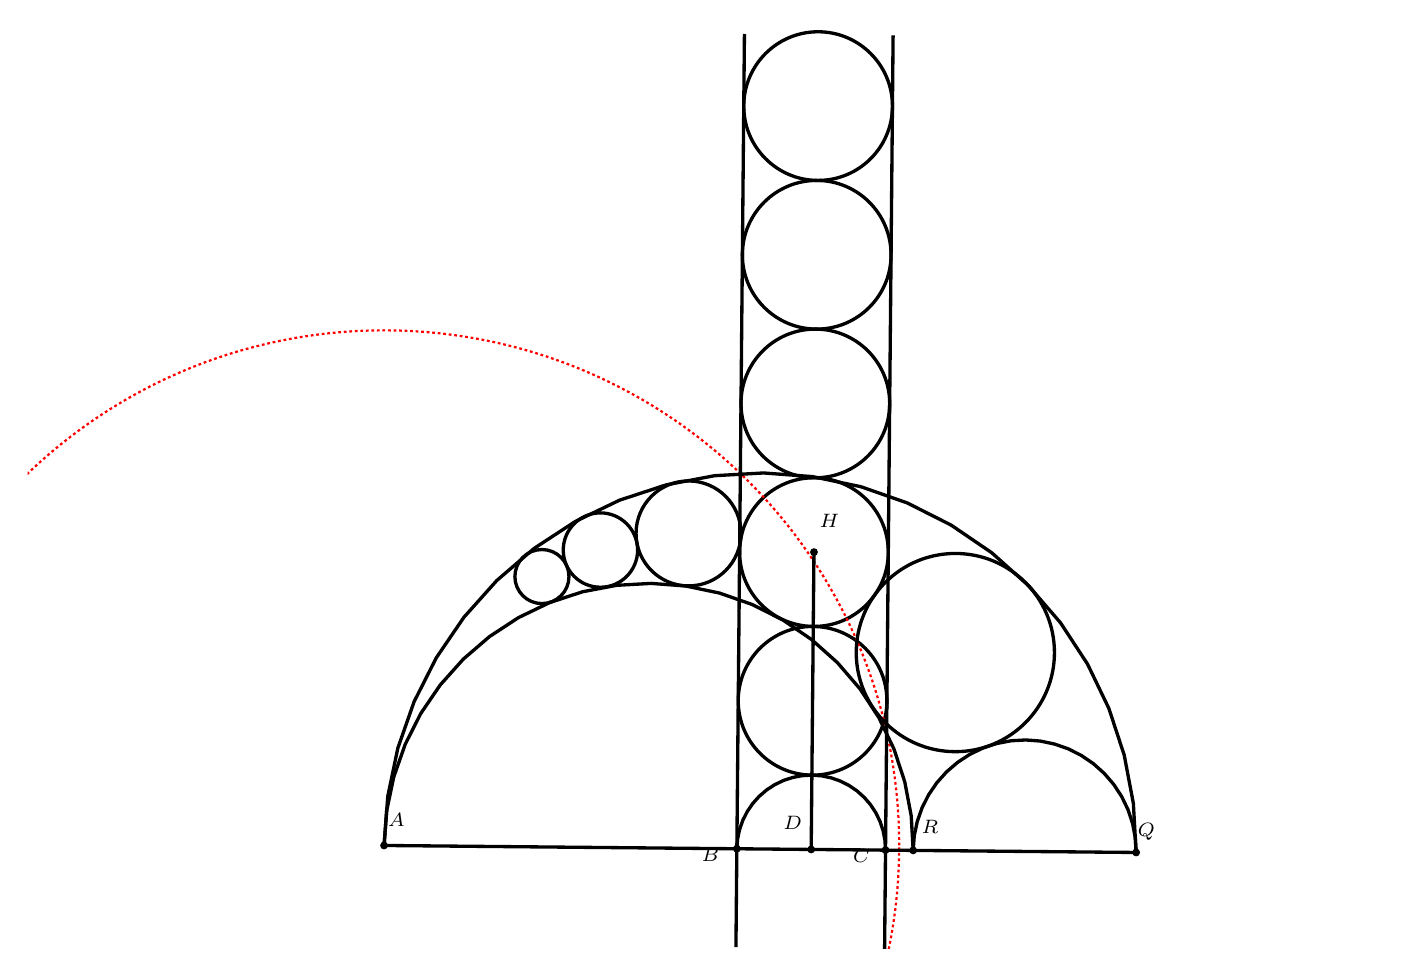
\begin{tikzpicture}[scale=0.8][line cap=round,line join=round,>=triangle 45,x=1cm,y=1cm]
\clip(-10.821034530821956,-4.356345156636261) rectangle (10.956341358104297,10.258693773265371);
\draw [line width=1.2pt] (1.6392365597850376,-0.42681440164616585) circle (1.1801042099412027cm);
\draw [line width=1.2pt] (1.661191037071024,1.9332919065973635) circle (1.180104209941203cm);
\draw [line width=1.2pt] (1.6831455143570102,4.293398214840894) circle (1.1801042099412047cm);
\draw [line width=0.8pt,dash pattern=on 1pt off 1pt,color=ffqqqq] (-5.163335827323846,-2.7238451944494817) circle (8.17743523083328cm);
\draw [line width=1.2pt] (-0.3300271381104034,2.2300138539887073) circle (0.8331006319058871cm);
\draw [line width=1.2pt] (3.9057009675370535,0.33850469224027746) circle (1.5732884404153449cm);
\draw [line width=1.2pt] (1.7050999916429965,6.653504523084423) circle (1.1801042099412007cm);
\draw [line width=1.2pt] (-1.7285158773110325,1.965651619233705) circle (0.5901555449068558cm);
\draw [line width=1.2pt] (1.7270544689289826,9.013610831327943) circle (1.180104209941199cm);
\draw [line width=1.2pt] (-2.65718028732941,1.5452729802408975) circle (0.4292245542496005cm);
\draw [line width=1.2pt] (-5.163335827323846,-2.7238451944494817)-- (6.775578166883001,-2.8349048595118713);
\draw [line width=1.2pt] (0.4226975774087187,-4.3380637003677815)-- (0.5575465709430273,10.158203104570411);
\draw [line width=1.2pt] (2.917647376166211,10.135657052597308)-- (2.7825913588425233,-4.382864809699166);
\draw [shift={(0.8061211697795776,-2.7793750269806763)},line width=1.2pt]  plot[domain=-0.009302057275135667:3.1322905963146574,variable=\t]({1*5.969715269807092*cos(\t r)+0*5.969715269807092*sin(\t r)},{0*5.969715269807092*cos(\t r)+1*5.969715269807092*sin(\t r)});
\draw [shift={(-0.9636483637792066,-2.7629120545754784)},line width=1.2pt]  plot[domain=-0.009302057275135667:3.1322905963146574,variable=\t]({1*4.199869165940067*cos(\t r)+0*4.199869165940067*sin(\t r)},{0*4.199869165940067*cos(\t r)+1*4.199869165940067*sin(\t r)});
\draw [shift={(5.005808633324217,-2.818441887106673)},line width=1.2pt]  plot[domain=-0.009302057275135667:3.132290596314657,variable=\t]({1*1.7698461038670255*cos(\t r)+0*1.7698461038670255*sin(\t r)},{0*1.7698461038670255*cos(\t r)+1*1.7698461038670255*sin(\t r)});
\draw [shift={(1.6172820824990513,-2.786920709889695)},line width=1.2pt]  plot[domain=-0.009302057275135667:3.1322905963146574,variable=\t]({1*1.1801042099412027*cos(\t r)+0*1.1801042099412027*sin(\t r)},{0*1.1801042099412027*cos(\t r)+1*1.1801042099412027*sin(\t r)});
\draw [line width=1.2pt] (1.661191037071024,1.9332919065973635)-- (1.6172820824990513,-2.786920709889695);
\begin{scriptsize}
\draw [fill=black] (-5.163335827323846,-2.7238451944494817) circle (1.5pt);
\draw[color=black] (-4.965340125132897,-2.311691531509295) node {$A$};
\draw [fill=black] (0.4372289283772869,-2.7759434712467015) circle (1.5pt);
\draw[color=black] (0.01925924499911158,-2.8682244708929665) node {$B$};
\draw [fill=black] (2.7973352366208157,-2.797897948532688) circle (1.5pt);
\draw[color=black] (2.4147705927809993,-2.8924215552139954) node {$C$};
\draw [fill=black] (1.6172820824990513,-2.786920709889695) circle (1.5pt);
\draw[color=black] (1.3259017983346868,-2.360085700151353) node {$D$};
\draw [fill=black] (1.661191037071024,1.9332919065973635) circle (1.5pt);
\draw[color=black] (1.9066318220393867,2.430936995412427) node {$H$};
\draw [fill=black] (6.775578166883001,-2.8349048595118713) circle (1.5pt);
\draw[color=black] (6.939625360813453,-2.5052682060775284) node {$Q$};
\draw [fill=black] (3.2360390997654327,-2.8019789147014746) circle (1.5pt);
\draw[color=black] (3.503639387227312,-2.432676953114441) node {$R$};
\end{scriptsize}
\end{tikzpicture}

%ajouter des figures.
\end{sol}

%9
\begin{sol}

On commence par réécrire l'énoncé de la manière suivante : On suppose seulement que $P$ et $Q$ sont sur le cercle $\Gamma$ mais cette fois-ci les trois droites $(PQ)$, $(QR)$ et $(RP)$ sont tangentes au cercle inscrit.
On effectue comme dans l'exercice $3$ l'inversion depuis $\omega$ et on rajoute les points $D$, $E$ et $F$. L'inversion envoie $A$, $B$ et $C$ sur les points $X$, $Y$ et $Z$ qui sont les milieux du triangle $DEF$, le cercle circonscrit à $XYZ$ est donc de rayon la moitié de celui de $\omega$, il en est de même de l'image du cercle circonscrit de $PQR$ par l'inversion depuis $\omega$. Comme celui-ci à déjà deux points en commun avec le cercle d'Euler du triangle $DEF$ on en déduit que c'est celui-ci (il y en a en fait deux mais on peut éliminer l'autre (exercice)). On en déduit que $R$ est également sur le cercle circonscrit de $ABC$.
\end{sol}

%10
\begin{sol}

On regarde la composition de l'inversion de centre $A$ et de rayon $\sqrt{AB \cdot AC}$ avec la symétrie d'axe la bissectrice intérieure de l'angle en $A$. Cette inversion un peu spéciale est en fait une involution projective complexe. Elle envoie $B$ sur $C$ et $A$ sur l'infini. Elle échange les droites $AB$ et $AC$ ainsi que $\Gamma$ et $(BC)$. Finalement elle échange le cercle $A$-exinscrit et le cercle $A$-mixtilinéaire. Elle envoie donc le point $S$ sur le point $T$. Cette involution échange donc les droites $(AS)$ et $(AT)$ ce qui montre bien que la bissectrice de ces deux droites est la bissectrice de $\widehat{BAC}$ cela conclut.
\end{sol}

%11
\begin{sol}

On note $\Gamma$ le cercle circonscrit de $ABC$.
Comme dans l'exercice précédent on va composer une inversion de centre $A$ avec une symétrie axiale par rapport à la bissectrice en $A$. On opère cette involution $I$ de sorte que $B$ soit échangé avec $M_B$, comme $(M_BM_C)$ est parallèle à $(BC)$, on a alors $AB\cdot AM_B=AC \cdot AM_C$, donc $C$ est envoyé sur $M_C$.
On note $A'$ le point diamétralement opposé à $A$ dans le cercle circonscrit à $ABC$. Alors $O$ est le milieu de $[AA']$, ainsi si on note $A^*$ l'image de $A'$ par $I$, on obtient que l'image $O^*$ de $O$ par $I$ s'obtient par une homothétie du point $A^*$ de facteur 2 depuis $A$. Comme $(AA')\perp \Gamma$ on a $(AA^*)\perp (M_BM_C)$. et finalement $A^*$ est le pied de la hauteur issue de $A$ dans $AM_BM_C$. $O^*$ est alors le pied de la hauteur issue de $A$ dans $ABC$. Il se situe sur le cercle circonscrit à $M_AM_BM_C$. Les cercles circonscrits de $BOC$ et $M_AM_BM_C$ sont échangés par $I$, donc $E$ et $F$ également. $(AE)$ et $(AF)$ sont échangées et la conclusion suit.
\end{sol}

%12
\begin{sol}

Les quatre cercles se recoupent en un point $M$, le point de Miquel du quadrilatère, une involution depuis $M$ échange $B$ et $D$ ainsi que $A$ et $C$. Les quatre cercles sont alors envoyés sur les quatre côtés du quadrilatère qui sont bient tous tangents à un même cercle.
\end{sol}

%13
\begin{sol}

\definecolor{ududff}{rgb}{0.30196078431372547,0.30196078431372547,1}
\begin{tikzpicture}[line cap=round,line join=round,>=triangle 45,x=1cm,y=1cm]
\clip(14.084792830217776,-6.584753910009965) rectangle (29.028481037350453,3.4441212867768307);
\draw [line width=1.2pt] (-1.8562097404188893,2.8572581782257145) circle (1.761105520950733cm);
\draw [line width=1.2pt] (1.609757227259506,2.2303262818806173) circle (1.7611055209507338cm);
\draw [line width=1.2pt] (3.6172581782257143,-0.6637902595811119) circle (1.7611055209507347cm);
\draw [line width=1.2pt] (2.9903262818806176,-4.129757227259504) circle (1.761105520950732cm);
\draw [line width=1.2pt] (0.09620974041888537,-6.137258178225714) circle (1.7611055209507367cm);
\draw [line width=1.2pt] (-3.3697572272595067,-5.510326281880617) circle (1.761105520950735cm);
\draw [line width=1.2pt] (-5.377258178225714,-2.616209740418891) circle (1.7611055209507311cm);
\draw [line width=1.2pt] (-4.750326281880616,0.8497572272595091) circle (1.7611055209507374cm);
\draw [line width=1.2pt] (-0.88,-1.64) circle (2.8408849808763605cm);
\draw [line width=1.2pt] (-0.88,-1.64) circle (6.363096022777828cm);
\draw [line width=2pt] (49.814144202758705,-2.1408403179873314) circle (38.64492952810329cm);
\draw [line width=1.2pt] (21.14603705350571,0.6322396456128585) circle (0.9771088820347238cm);
\draw [line width=1.2pt] (19.044868710058307,0.6493129808024323) circle (1.1241288261458617cm);
\draw [line width=1.2pt] (17.47268896135121,-1.1067890547074926) circle (1.232912438101927cm);
\draw [line width=1.2pt] (17.931889515948466,-3.495090318691454) circle (1.1991336299012776cm);
\draw [line width=1.2pt] (19.93166239696527,-4.542848472356283) circle (1.0584953750996196cm);
\draw [line width=1.2pt] (21.815327282370568,-3.9147158344912234) circle (0.9271390351734023cm);
\draw [line width=1.2pt] (22.729459856315415,-2.3741235867405432) circle (0.8642466956440895cm);
\draw [line width=1.2pt] (22.497727225423287,-0.6436680952612626) circle (0.8816559992994097cm);
\draw [line width=1.2pt] (20.26460265854544,-1.8489012387084616) circle (1.655947646122197cm);
\draw [line width=1.2pt] (19.885915998402897,-1.845159947672464) circle (3.7565717471084277cm);
\end{tikzpicture}

On opère une inversion qui envoie les cercles $\omega$ et $\Omega$ sur des cercles concentriques : on obtient alors la figure suivante : 

\definecolor{ududff}{rgb}{0.30196078431372547,0.30196078431372547,1}
\begin{tikzpicture}[scale=0.6][line cap=round,line join=round,>=triangle 45,x=1cm,y=1cm]
\clip(-11.365021653800731,-11.389102163694476) rectangle (18.411136713707457,8.594008562944332);
\draw [line width=1.2pt] (-1.8562097404188893,2.8572581782257145) circle (1.761105520950733cm);
\draw [line width=1.2pt] (1.609757227259506,2.2303262818806173) circle (1.7611055209507338cm);
\draw [line width=1.2pt] (3.6172581782257143,-0.6637902595811119) circle (1.7611055209507347cm);
\draw [line width=1.2pt] (2.9903262818806176,-4.129757227259504) circle (1.761105520950732cm);
\draw [line width=1.2pt] (0.09620974041888537,-6.137258178225714) circle (1.7611055209507367cm);
\draw [line width=1.2pt] (-3.3697572272595067,-5.510326281880617) circle (1.761105520950735cm);
\draw [line width=1.2pt] (-5.377258178225714,-2.616209740418891) circle (1.7611055209507311cm);
\draw [line width=1.2pt] (-4.750326281880616,0.8497572272595091) circle (1.7611055209507374cm);
\draw [line width=1.2pt] (-0.88,-1.64) circle (2.8408849808763605cm);
\draw [line width=1.2pt] (-0.88,-1.64) circle (6.363096022777828cm);
\draw [line width=1.2pt] (25.748622576293975,0.18702930690610486) circle (0.820236746346545cm);
\draw [line width=1.2pt] (23.98479101438375,0.20136156522722226) circle (0.943653043980289cm);
\draw [line width=1.2pt] (22.665020387525804,-1.2728031326309006) circle (1.0349717471127988cm);
\draw [line width=1.2pt] (23.050497559772,-3.2776692167321917) circle (1.0066160333910386cm);
\draw [line width=1.2pt] (24.729212421048825,-4.157212689032306) circle (0.8885568624518179cm);
\draw [line width=1.2pt] (26.310460105129515,-3.6299250134933994) circle (0.7782894205586413cm);
\draw [line width=1.2pt] (27.07783121593195,-2.3366706014463876) circle (0.7254942726543234cm);
\draw [line width=1.2pt] (26.883302619702768,-0.8840349657199316) circle (0.7401085606307696cm);
\draw [line width=1.2pt] (25.008700042036978,-1.8957712525824006) circle (1.3900898194140279cm);
\draw [line width=1.2pt] (24.690810480585718,-1.8926306155020052) circle (3.1534645154889436cm);

\end{tikzpicture}

sur laquelle l'exercice est alors immédiat par symétrie.
\end{sol}


%14
\begin{sol}

On note $S$ le pôle sud. On va faire l'inversion $I_S$ de centre $S$ et de rayon $SI=SA=SB$ (donc par rapport au cercle antarctique). On veut montrer que $\omega'$ le cercle circonscrit de $XYZ$ est échangé avec $\omega$ par l'inversion $I_S$. Les points $X$ et $Y$ sont fixes par cette inversion. Il suffit de montrer que $I_S$ envoie $Z$ sur un point de $\omega$. Pour cela on se rend compte que beaucoup de points de la figure deviennent inutiles. On peut ainsi garder uniquement les points $Z$, $S$ et $I$ ainsi que les deux cercles $\omega$ et $\gamma$.

On remarque alors que la figure est connue, les points de tangence $P$ et $Q$ (comme sur la figure) ainsi que le point $Z$ forment un triangle dont le cercle inscrit est $\omega$ et dont le cercle antarctique est $\gamma$. Cela conclut alors avec l'exercice 2. 
\end{sol}

%15
\begin{sol}
 
On va effectuer $\mathcal{I}$ l'inversion par rapport au cercle $\omega$. On note $E$, $F$, $G$ et $H$ les points de tangence de $\omega$ avec $(AB)$, $(BC)$, $(CD)$ et $(DA)$ respectivement. Alors par $\mathcal{I}$, les points $A$, $B$, $C$ et $D$ sont envoyés sur les milieux des côtés du quadrilatère $EFGH$. On note avec des $^*$ ces inverses. Le cercle $\omega_1$ est envoyé sur la droite $(A^*C^*)$ et les tangentes sont envoyés sur des cercles passant par $I$ et $A^*$ (ou $C^*$) et tangent à $(A^*C^*)$ en $A^*$ (ou $C^*$). Le point $X^*$ est alors la deuxième intersection de ces deux cercles. Par axes radicaux, les points $I$, $X^*$ et le milieu de $[A^*C^*]$ sont concourants. De même, $I$, $Y^*$ et le milieu de $[B^*D^*]$ sont alignés. Mais par des résutats connus sur les barycentres, les milieux de $[A^*C^*]$ et $[B^*D^*]$ sont les mêmes.
\end{sol}

\subsubsection{Solutions des exos durs}

%16
\begin{sol}



On montre d'abord le lemme suivant : 

\begin{lem}

Soit $\omega$ un cercle, $A$, $A'$, $B$, $B'$, $C$ et $C'$ des points sur $\omega$. Soit de plus $P$ un point qui n'est pas sur le cercle. Alors les cercles circonscrits des triangles $PAA'$, $PBB'$ et $PCC'$ se coupent en un deuxième point $Q$ si et seulement si les droites $(AA')$, $(BB')$ et $(CC')$ sont concourantes au point $R$.
\end{lem}

\begin{preuve}
On peut donner beaucoup de preuves de ce théorème, on va ici le démontrer de manière élémentaire.

On suppose dans un premier temps que les trois cercles s'intersectent en $Q$, alors les droites $(PQ)$, $(AA')$ et $(BB')$ sont les trois axes radicaux des cercles $\omega$, $PAA'$ et $PBB'$ et sont donc concourant en $R$, par symétrie la droite $(CC')$ passe également par $R$.


Dans l'autre sens en supposant l'intersection en $R$, on voit que $R$ est sur l'axe radical des cercles circonscrits aux triangles $PAA'$ et $PBB'$ il est donc sur la droite $(PQ)$ où $Q$ est la deuxième intersection des deux cercles. Par symétrie, $Q$ est également sur le cercle circonscrit au triangle $PCC'$.
\end{preuve}

On peut maintenant résoudre l'exercice. On opère l'inversion qui envoie $\omega$ et $\Omega$ sur deux cercles concentriques. On obtient comme précédemment (exercice 13) une figure très symétrique. Soit $P$ le centre de l'inversion et on note avec une $^*$ les inverses des points. Pour conclure il faut montrer que les cercles circonscrits des triangles de la forme $PT_i^*T_{i+4}^*$ se coupent en un point autre que $P$, d'après le lemme il suffit en fait de montrer que les droites $(T_i^*T_{i+4}^*)$ sont concourantes ce qui est évident.
\end{sol}

%17
\begin{sol}



On va utiliser le premirer théorème de Desargues. Pour cela on se restreint à démontrer seulement la concourance des droites $(O_0O_4)$, $(O_1O_5)$ et $(O_2O_6)$. Il faut alors montrer que les triangles $O_0O_2O_5$ et $O_1O_4O_6$ sont perspectifs. Ce qui revient à montrer que les intersections suivantes sont alignés : $(O_1O_6)\cap(O_2O_5)$, $(O_1O_4)\cap (O_0O_5)$ et $(O_0O_2)\cap (O_6O_4)$. On va en fait montrer que ces points sont des centres d'homothétie et qu'ils sont alignés. Pour montrer cela on va juste montrer que les bissectrices des cercles $\omega_i$ ont deux points en commun.

On utilise le lemme suivant : 

\begin{lem}
Soit $\omega$ et $\gamma$ deux cercles et $k$ leur bissectrice. Soit $\mathcal{I}$ une inversion, on note par $^*$ les images après inversion. Alors $\omega^*$ et $\gamma^*$ ont pour bissectrice $k^*$.
\end{lem}

Pour cela on va commencer par effectuer une inversion $\mathcal{I}$ qui envoie $\omega$ et $\Omega$ sur deux cercles concentriques. Dans ce cas la figure devient très symétrique et les bissectrices des cercles deviennent des droites qui passent par le centre commun de $\omega^*$ et $\Omega^*$. Alors ils passent tous par le même point. En réappliquant $\mathcal{I}$ on se retrouve avec des bissectrices qui passent par les deux mêmes points. De plus, on remarque que les paires des cercles $\omega_1$ et $\omega_6$ ainsi que $\omega_2$ et $\omega_5$ ont la même bissectrice après inversion donc aussi avant inversion (d'après le lemme). Ainsi, $(O_1O_6)\cap(O_2O_5)$ est le centre d'homothetie commun des deux pairs. Commes les bissectrices passent toutes par les deux même points les centre de ces cercles (qui sont les centres d'homothétie) sont tous alignés ce qui conclut.
\end{sol}

%18
\begin{sol}

\definecolor{ffqqqq}{rgb}{1,0,0}
\definecolor{ududff}{rgb}{0.30196078431372547,0.30196078431372547,1}
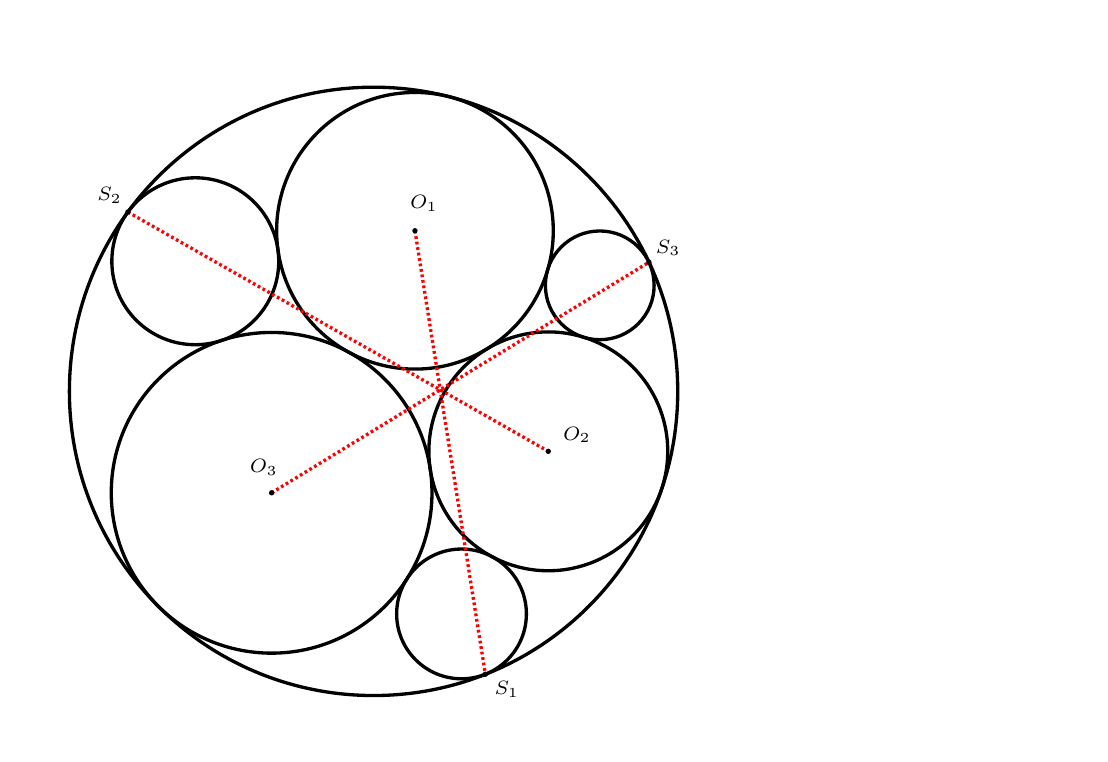
\begin{tikzpicture}[scale=0.5][line cap=round,line join=round,>=triangle 45,x=1cm,y=1cm]
\clip(22.513135358172878,-9.830806232177157) rectangle (49.23016296748206,8.099287852292502);
\draw [line width=2pt] (-8.2468915983988,-5.306220915011429) circle (6.047351718718782cm);
\draw [line width=2pt] (-2.0191075360266852,5.061833719876833) circle (6.047351718718784cm);
\draw [line width=2pt] (3.8459991344254867,-5.515612804865403) circle (6.047351718718785cm);
\draw [line width=2pt] (-2.14,-1.92) circle (13.030232004092056cm);
\draw [line width=2pt] (-10.807837340852949,3.2865137721161006) circle (2.9188923388093535cm);
\draw [line width=2pt] (-2.3150545213796145,-12.02982421910806) circle (2.9188923388093535cm);
\draw [line width=2pt] (6.702891862232562,2.983310446991955) circle (2.9188923388093535cm);
\draw [line width=2pt] (80,0) circle (62.464925722018cm);
\draw [line width=1.2pt] (35.73682608858236,-2.6615122064856287) circle (3.0332510979232836cm);
\draw [line width=1.2pt] (32.34979213756566,2.9407468108728807) circle (3.5132979993427433cm);
\draw [line width=1.2pt] (28.709089512341073,-3.714851477840376) circle (4.072985951712617cm);
\draw [line width=1.2pt] (31.298398242257782,-1.1383866006192482) circle (7.725750789801296cm);
\draw [line width=1.2pt] (37.04348961048301,1.5546803792637252) circle (1.3807776151226179cm);
\draw [line width=1.2pt] (33.53240457964263,-6.790944961912673) circle (1.647741218954618cm);
\draw [line width=1.2pt] (26.770194220504337,2.166538895024939) circle (2.119757194158961cm);
\draw [line width=1.2pt,dash pattern=on 1pt off 1pt,color=ffqqqq] (28.709089512341073,-3.714851477840376)-- (38.29372240732715,2.140739059021125);
\draw [line width=1.2pt,dash pattern=on 1pt off 1pt,color=ffqqqq] (25.057974452862695,3.416208463145148)-- (35.73682608858236,-2.6615122064856287);
\draw [line width=1.2pt,dash pattern=on 1pt off 1pt,color=ffqqqq] (32.34979213756566,2.9407468108728807)-- (34.13804106023838,-8.323346860245362);
\begin{scriptsize}
\draw[color=black] (48.96299269138897,52.909680270350364) node {$k_1$};
\draw [fill=black] (28.709089512341073,-3.714851477840376) circle (1.5pt);
\draw[color=black] (28.50962377715116,-3.077335364268469) node {$O_3$};
\draw [fill=black] (32.34979213756566,2.9407468108728807) circle (1.5pt);
\draw[color=black] (32.576549091012666,3.6316071242913694) node {$O_1$};
\draw [fill=black] (35.73682608858236,-2.6615122064856287) circle (1.5pt);
\draw[color=black] (36.46536088747878,-2.2461389497566304) node {$O_2$};
\draw [fill=black] (25.057974452862695,3.416208463145148) circle (1.5pt);
\draw[color=black] (24.59112639445248,3.839406227919329) node {$S_2$};
\draw [fill=black] (38.29372240732715,2.140739059021125) circle (1.5pt);
\draw[color=black] (38.78083661361891,2.5035548474538745) node {$S_3$};
\draw [fill=black] (34.13804106023838,-8.323346860245362) circle (1.5pt);
\draw[color=black] (34.68422571352484,-8.717596748455945) node {$S_1$};
\end{scriptsize}
\end{tikzpicture}

On procède comme dans l'exercice précédent. On montre que le centre d'homothétie de $\omega_1$ et $\omega_3$ est le même que celui de $\gamma_1$ et $\gamma_3$. Ce qui est clair après inversion depuis $S_2$, les details sont laissés au lecteur.


\end{sol}

%19
\begin{sol}

\definecolor{qqffqq}{rgb}{0,1,0}
\definecolor{ffqqqq}{rgb}{1,0,0}
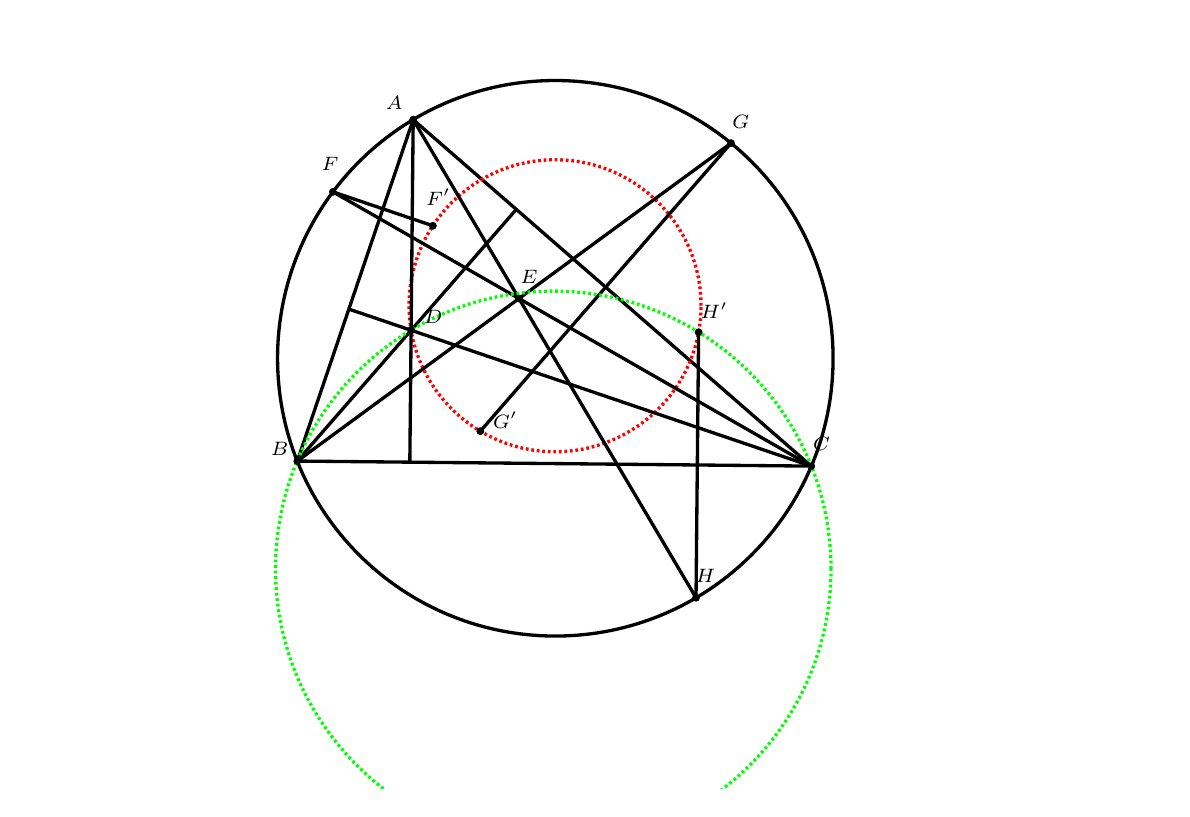
\begin{tikzpicture}[scale=0.8][line cap=round,line join=round,>=triangle 45,x=1cm,y=1cm]
\clip(-9.22,-9.28) rectangle (8.78,2.8);
\draw [line width=1.2pt] (-3.1,1.34)-- (-4.94,-4.08);
\draw [line width=1.2pt] (-4.94,-4.08)-- (3.22,-4.16);
\draw [line width=1.2pt] (3.22,-4.16)-- (-3.1,1.34);
\draw [line width=1.2pt] (-0.8436110910795415,-2.448331290113219) circle (4.40939280082305cm);
\draw [line width=1.2pt,dash pattern=on 1pt off 1pt,color=ffqqqq] (-0.8479956515042245,-1.6142892754408873) circle (2.317668657556315cm);
\draw [line width=1.2pt] (1.3899556039539487,-6.250163044779293)-- (1.4312870167292557,-2.0343589416979944);
\draw [line width=1.2pt] (1.9455723473545006,0.9668115500496053)-- (-2.0336770581993178,-3.605707766877691);
\draw [line width=1.2pt] (-4.374005371849363,0.1934599761032989)-- (-2.787320978022454,-0.345193028443106);
\draw [line width=1.2pt] (-4.374005371849363,0.1934599761032989)-- (3.22,-4.16);
\draw [line width=1.2pt] (1.9455723473545006,0.9668115500496053)-- (-4.94,-4.08);
\draw [line width=1.2pt] (-3.1,1.34)-- (1.3899556039539487,-6.250163044779293);
\draw [line width=1.2pt] (-1.462996791675452,-0.08460722243433728)-- (-4.94,-4.08);
\draw [line width=1.2pt] (-4.121103961907088,-1.6678171051828334)-- (3.22,-4.16);
\draw [line width=1.2pt] (-3.153308986064393,-4.097516578567997)-- (-3.1,1.34);
\draw [line width=1.2pt,dash pattern=on 1pt off 1pt,color=qqffqq] (-0.8763889089204587,-5.791668709886782) circle (4.40939280082305cm);
\begin{scriptsize}
\draw [fill=black] (-3.1,1.34) circle (1.5pt);
\draw[color=black] (-3.4,1.61) node {$A$};
\draw [fill=black] (-4.94,-4.08) circle (1.5pt);
\draw[color=black] (-5.22,-3.89) node {$B$};
\draw [fill=black] (3.22,-4.16) circle (1.5pt);
\draw[color=black] (3.38,-3.81) node {$C$};
\draw [fill=black] (-3.1327778178409176,-2.0033374197735627) circle (1.5pt);
\draw[color=black] (-2.78,-1.79) node {$D$};
\draw [fill=black] (-1.42,-1.5) circle (1.5pt);
\draw[color=black] (-1.26,-1.15) node {$E$};
\draw [fill=black] (-4.374005371849363,0.1934599761032989) circle (1.5pt);
\draw[color=black] (-4.42,0.63) node {$F$};
\draw [fill=black] (1.9455723473545006,0.9668115500496053) circle (1.5pt);
\draw[color=black] (2.1,1.31) node {$G$};
\draw [fill=black] (1.3899556039539487,-6.250163044779293) circle (1.5pt);
\draw[color=black] (1.54,-5.91) node {$H$};
\draw [fill=black] (1.4312870167292557,-2.0343589416979944) circle (1.5pt);
\draw[color=black] (1.68,-1.69) node {$H'$};
\draw [fill=black] (-2.0336770581993178,-3.605707766877691) circle (1.5pt);
\draw[color=black] (-1.64,-3.43) node {$G'$};
\draw [fill=black] (-2.787320978022454,-0.345193028443106) circle (1.5pt);
\draw[color=black] (-2.7,0.11) node {$F'$};
\end{scriptsize}
\end{tikzpicture}

On va utiliser le lemme suivant : 

\begin{lem}

Soit $A$, $A'$, $B$, $B'$, $C$ et $C'$ des affixes complexes. Soit $\mathcal{I}$ une inversion. Alors $\dfrac{A-C'}{B-C'}\dfrac{B-A'}{C-A'}\dfrac{C-B'}{A-B'}$ est conjugué par $\mathcal{I}$ (c'est un nombre complexe).
\end{lem}

\begin{preuve}
Pour la preuve il suffit de calculer avec $\dfrac{1}{\overline{A}}$.
\end{preuve}

On va maintenant regarder la quantité précédente mais avec les points $A$, $A^*$, $B$, $B^*$, $C$ et $C^*$. On peut maintenant opérer l'inversion de centre $H$ de l'exercice 1. Le module de $\dfrac{A-C*}{B-C^*}\dfrac{B-A^*}{C-A^*}\dfrac{C-B^*}{A-B^*}$ est 1 car c'est le même que celui de $\dfrac{A-C'}{B-C'}\dfrac{B-A'}{C-A'}\dfrac{C-B'}{A-B'}$ qui est 1 par Ceva. Après inversion c'est le même module. Comme les points $A^*$, $B^*$ et $C^*$ se retrouvent sur les côtés du triangle $H_AH_BH_C$ avec des rapport 1 ce qui est alors l'énoncé de Menalaüs. Cela montre l'alignement de ces points et donc la cocyclicité avant inversion.


\end{sol}

%20
\begin{sol}

On va commencer par quelques motivations.

\begin{lem}
Soit $ABC$ un triangle, on note $I$ le centre du cercle inscrit du triangle ainsi que $I_A$ le centre du cercle $A$-exinscrit. On note $\mathcal{I}$ l'involution de centre $A$ composée avec la symétrie d'axe la bissectrice de $\widehat{BAC}$ qui envoie $B$ sur $C$. Cette involution échange $I_A$ et $I$.
\end{lem}

\begin{preuve}
On note $\omega$ le cercle antarctique du triangle $ABC$. Ce cercle a pour axe de symétrie la bissectrice de $\widehat{BAC}$, ainsi la puissance de $A$ par rapport à ce cercle est $AB\cdot AC$, donc il est fixe par l'involution $\mathcal{I}$. Il suit que $I$ et $I_A$ sont échangés par $\mathcal{I}$.
\end{preuve}

\begin{lem}
Même notation que dans le lemme précédent. On veut maintenant montrer que $\mathcal{I}$ échange $O$ et $A'$, avec $O$ le centre du cercle circonscrit du triangle $ABC$ et $A'$ le symétrique de $A$ par la droite $(BC)$.
\end{lem}

\begin{preuve}
On note $A''$ le point diamétralement opposé à $A$ sur le cercle circonscrit du triangle $ABC$. Comme la droite $(AA'')$ est perpendiculaire au cercle circonscrit du triangle $ABC$, après inversion elle devient perpendiculaire à $(BC)$ et donc $A''$ est envoyé sur le pied de la hauteur issue de $A$. Ainsi par un peu de calcul $O$ est envoyé sur $A'$.
\end{preuve}

En combinant les deux lemmes avec le fait que le symétrique de $H$ par rapport à la droite $(BC)$ soit sur le cercle circonscrit du riangle $ABC$ on obtient le corollaire suivant : 

\begin{cor}
Soit $ABC$ un triangle, $O$ est le centre du cercle circonscrit et $H$ est l'orthocentre. Alors soit $\mathcal{I}$ l'involution standart de centre $A$, on a
$\mathcal{I}$ fixe le cercle antarctique et échange les cercles circonscrits des triangle $BOC$ et $BHC$. 
\end{cor}

Supposons ici dans un premier temps que les droites $(AB)$ et $(CD)$ sont parallèles. On peut regarder l'involution de centre $P$ qui envoie $A$ sur $C$ et $B$ sur $D$ (c'est possible comme les droites $(AB)$ et $(CD)$ sont supposées parallèles). Dans ce cas d'après le corollaire précédent on obtient que cette involution échange les cercles circonscrits des triangles $BOA$ et $DHC$ de même avec $BI_1A$ et $DI_2C$. Dans ce cas l'exercice est donc terminé (par conservation du parallèlisme).

Malheureusement, on ne dispose pas de l'hypothèse de parallèlisme dans l'énoncé, il va donc falloir faire sans. On introduit donc $M$ le point de Miquel du quadrilatère formé par les droites $(AB)$, $(BC)$, $(CD)$ et $(DA)$. On va regarder $\mathcal{I}$ l'involution depuis $M$ qui échange $A$ avec $C$ et $B$ avec $D$. On veut ensuite montrer que, comme dans le premier cas, que l'involution $\mathcal{I}$ échange les cercles circonscrits des triangles $BOA$ et $DHC$ de même avec $BI_1A$ et $DI_2C$. On remarque alors que $BI_1A$ est le cercle antarctique de $ABM$ également, ce qui implique qu'il sera envoyé sur le cercle antarctique de $CDM$ qui est bien $DI_2C$. Pour les autres cercles on peut remarque que $O$ reste le centre du cercle circonscrit du triangle $AMB$, et que $HDC$ est le symétrique du cercle circonscrit du triangle $DPC$ (ou bien $DMC)$ par rapport à la droite $(DC)$ ce qui montre que $DHC$ passe également par l'orthocentre du triangle $DMC$ cela conclut l'échange des cercles circonscrits aux triangles $BOA$ et $DHC$.

\end{sol}


%21
\begin{sol}

On renvoie vers la solution officielle de cet exercice.
\end{sol}

%22
\begin{sol}

On renvoie vers la solution officielle de cet exercice.
\end{sol}
